\documentclass[a4paper]{article}    % define document layout
%\documentclass[draft]{article}     % use draft option in packages
%-----------------------------
% preamble
%-----------------------------
\usepackage[sumlimits,]{amsmath}    % math equations and formulas
\usepackage[utf8]{inputenc}         % use UTF-8 encoding
\usepackage[english]{babel}         % use English language
\usepackage{graphicx}              % insert images
%\usepackage[draft]{graphicx}        % do not render figures
\usepackage{subcaption}             % multiple images in one figure
\usepackage{hyperref}               % hyperlinks
\usepackage{float}                  % floating objects (figures, tables)
\usepackage{geometry}               % page size and margins
\geometry{a4paper, margin=1in}      % margins
\usepackage{ragged2e}               % text alignment
\usepackage[table]{xcolor}          % change cell color in tables
%\usepackage{multirow}               % merge rows in table
%\usepackage[thinc]{esdiff}          % macros for derivatives

\graphicspath{                      % path for figures
    {../figures/} 
}

%-----------------------------
% body
%-----------------------------
\begin{document}

\begin{figure}
    \centering
    % UNICAMP logo
    \begin{subfigure}{0.45\textwidth}
        \centering
        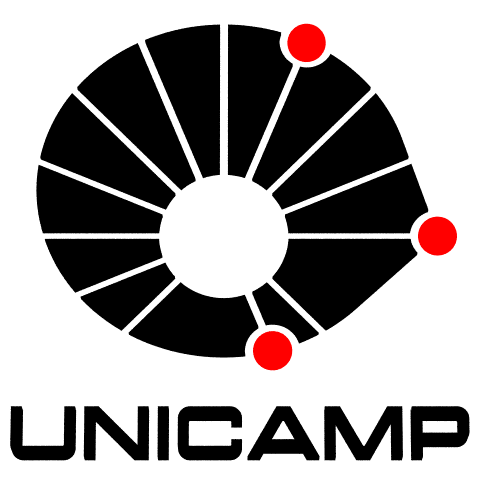
\includegraphics[width=1.5cm]{unicamp}
%        \label{fig:unicamp}
    \end{subfigure}
    \hfill
    % FEEC logo
    \begin{subfigure}{0.45\textwidth}
        \centering
        
\includegraphics[width=1.5cm]{feec}
%        \label{fig:feec}
    \end{subfigure}
\end{figure}

\title{
    \vspace{5cm}
    IA353A - Neural Networks\\
    EC1
    \vspace{1cm}
}
\author{
    Rafael Claro Ito\\
    (R.A.: 118430)
    \vspace{11cm}
}
%R.A.: 118430
%ito.rafael@gmail.com
\date{May 2020}
\maketitle
\newpage

%=================================================
\section*{Question 1}
%=================================================

\newpage

%=================================================
\section*{Question 2}
%=================================================

\[\|Ax-b\|_{P}^{2}+\|x-x_{0}\|_{Q}^{2}\]
%------------------------
\paragraph{Since we are searching for $x$ that minimizes the previous expression, we will calculate the derivative with relation to $x$ and set it equal to zero:}
    \[\frac{d}{dx} (\|Ax-b\|_{P}^{2}+\|x-x_{0}\|_{Q}^{2}) = 0\]
%------------------------
\paragraph{Property used: $\|x\|_{Q}^{2} = x^{T}Qx$}
    \[\frac{d}{dx} [\overbrace{(Ax-b)^{T} P (Ax-b)}^{\|Ax-b\|_{P}^{2}} + \overbrace{(x-x_0)^T Q (x-x_0)}^{\|x-x_{0}\|_{Q}^{2}}] = 0\]
%------------------------
\paragraph{Property used: $(M + N)^T = M^T + N^T$}
    \[\frac{d}{dx} \{[(Ax)^T-b^T] P (Ax-b) + (x^T-x_0^T) Q (x-x_0)\} = 0\]
%------------------------
\paragraph{Property used: $(MN)^T = N^T M^T$}
    \[\frac{d}{dx} \{[x^TA^T-b^T] P (Ax-b) + (x^T-x_0^T) Q (x-x_0)\} = 0\]
    \[\frac{d}{dx} [(x^TA^TPAx - x^TA^TPb -b^TPAx + b^TPb) + (x^TQx - x^TQx_0 - x_0^TQx + x_0^TQx_0)] = 0\]
%------------------------
\paragraph{Properties used:}
    \begin{itemize}
        \item $\frac{d}{dy}(y^TMy) = M^Ty + My$.
        \item $\frac{d}{dy}(y^TMy) = 2My$, if $M = M^T$ (i.e. $M$ is symmetric)
        \item $\frac{d(Ax)}{dx} = A$
        \item $\frac{d(x^TA)}{dx} = A^T$
        \item obs.: $A^TPA$ is symmetric, since $(A^TPA)^T = (PA)^T(A^T)^T = A^TP^TA$, but $P^T = P$, since P is symmetric. Then $A^TPA = (A^TPA)^T$
    \end{itemize}
\paragraph{Using the previous properties, we have:}
    \[\frac{d}{dx} [(x^TA^TPAx - x^TA^TPb -b^TPAx + b^TPb) + (x^TQx - x^TQx_0 - x_0^TQx + x_0^TQx_0)] = 0\]
    \[[2A^TPAx - (A^TPb)^T - b^TPA + 0] + [2Qx - (Qx_0)^T - x_0^TQ + 0] = 0\]
    \[2A^TPAx - (Pb)^T(A^T)^T - b^TPA + 2Qx - x_0^TQ^T - x_0^TQ = 0\]
    \[2A^TPAx - b^TP^TA - b^TPA + 2Qx - x_0^TQ - x_0^TQ = 0\]
    \[2A^TPAx - b^TPA - b^TPA + 2Qx - x_0^TQ - x_0^TQ = 0\]
    \[2A^TPAx - 2b^TPA + 2Qx - 2x_0^TQ = 0\]
    \[2A^TPAx + 2Qx = 2b^TPA + 2x_0^TQ\]
    \[A^TPAx + Qx = b^TPA + x_0^TQ\]
    \[(A^TPA + Q)^{-1}(A^TPA + Q)x = (A^TPA + Q)^{-1}(b^TPA + x_0^TQ)\]
    \[x = (A^TPA + Q)^{-1}(b^TPA + x_0^TQ)\]
    \[x = (A^TPA + Q)^{-1}(b^TP^TA + x_0^TQ^T)\]
    \[x = (A^TPA + Q)^{-1}[(Pb)^TA + (Qx_0)^T]\]
    \[x = (A^TPA + Q)^{-1}[(A^TPb)^T + (Qx_0)^T]\]
    \[\boxed{x = (A^TPA + Q)^{-1}(A^TPb + Qx_0)^T}\]
%------------------------
%\paragraph{Properties used:}
%    \begin{itemize}
%        \item Since $Q$ is symmetric, $(Qx_0)^T = Qx_0$
%        \item Since $P$ is symmetric, $(A^TPb)^T = (A^TPb)$
%    \end{itemize}
%\paragraph{Then:}
%    \[x = (A^TPA + Q)^{-1}[(A^TPb)^T + (Qx_0)^T]\]
%    \[x = (A^TPA + Q)^{-1}(A^TPb + Qx_0)\]
%------------------------
\newpage

%=================================================
\section*{Question 3}
%=================================================

%------------------------
\subsection*{a)}
%------------------------

%------------------------
\subsection*{b)}
%------------------------

%------------------------
\subsection*{c)}
%------------------------

\paragraph{We want to prove that $N$ may not be unique in $M=N^TN$. For this, lets consider the orthogonal matrix $Q$ and the new matrix that is the result by its multiplication with $N$, i.e., $QN$:}
    \[M = (QN)^T(QN) = (N^TQ^T)(QN) = N^T(Q^TQ)N\]

\paragraph{Since $Q$ is orthogonal, $Q^TQ$ is equal to the identity matrix $I$. Hence:}
    \[M= N^T(Q^TQ)N = N^TIN = N^TN\]

\paragraph{So if $M$ can be decomposed in $N^TN$, it can also be decomposed by $(QN)^T(QN)$, with $Q$ being an orthogonal matrix.}

%------------------------
\subsection*{d)}
%------------------------


\newpage

%=================================================
\section*{Question 4}
%=================================================

\paragraph{The Taylor series expansion of a function $f(x,y)$ in a neighborhood around $(x_0,y_0)$ is as follows:}
    \[f(x,y) \approx f(x_0,y_0) + \underbrace{f_x(x_0,y_0)(x-x_0)+f_y(x_0,y_0)(y-y_0)}_{\text{first order term}} + ...\]

\paragraph{Ignoring terms from second order and higher, and considering the linearized function given $f_L(x,y)=2x+py-8$, we have:}
    \[f_L(x,y) = f(x_0,y_0) + f_x(x_0,y_0)(x-x_0)+f_y(x_0,y_0)(y-y_0)\]

\paragraph{Taking $f(x,y) = x\sqrt y$, we have:}
\begin{itemize}
    \item $f_x(x,y) = \sqrt y$
    \item $f_y(x,y) = \frac{x}{2\sqrt y}$
\end{itemize}
    \[2x+py-8 = \underbrace{x_0\sqrt y_0}_{f(x_0,y_0)} + \underbrace{\sqrt y_0}_{f_x(x_0,y_0)}(x-x_0) + \underbrace{\frac{x_0}{2\sqrt y_0}}_{f_y(x_0,y_0)}(y-y_0)\]
    \[2x+py-8 = x_0\sqrt y_0 + x\sqrt y_0 - x_0\sqrt y_0 + \frac{x_0 y}{2\sqrt y_0} - \frac{x_0 y_0}{2\sqrt y_0}\]
    \[2x+py-8 =  \sqrt y_0 x + \left(\frac{x_0}{2\sqrt y_0}\right) y - \left(\frac{x_0 y_0}{2\sqrt y_0}\right)\]
    
    \paragraph{Now, if we compare the terms that only depend on $x$, that only depend on $y$ and the independent terms (that only depend on $x_0$ and $y_0$), we have:}
\begin{itemize}
    \item (i)   $ 2 = \sqrt y_0 \implies \boxed{y_0 = 4}$ 
    \item (ii)  $ p = \left(\frac{x_0}{2\sqrt y_0}\right) $
    \item (iii) $ 8 = \left(\frac{x_0 y_0}{2\sqrt y_0}\right) $
\end{itemize}

\paragraph{Substituting in (i) in (iii):}
    \[\frac{x_0 y_0}{2\sqrt y_0} = 8\]
    \[\frac{4 x_0}{2\cdot2} = 8\]
    \[\boxed{x_0 = 8}\]

\paragraph{Substituting in (ii):}
    \[p = \frac{x_0}{2\sqrt y_0}\]
    \[p = \frac{8}{2\cdot2}\]
    \[\boxed{p = 2}\]

    \paragraph{So the point from where the function was linearized is $(x_0,y_0) = (8,4)$ and the coefficient $p = 2$, then $f_L(x,y) = 2x + 2y -8$.}

\newpage
 
%=================================================
\section*{Question 5}
%=================================================

\newpage

%=================================================
\section*{Question 6}
%=================================================

O primeiro paper selecionado é de 2002 com 2173 citações. Esse paper foi publicado no JAMA (The Journal of the American Medical Association) que é um jornal da área médica com 48 publicações por ano pela AMA (American Medical Association).

title: Effects of Cognitive Training Interventions With Older Adults - A Randomized Controlled Trial
year: 2002
cited by: 2173
publication: JAMA
reference:

Ball K, Berch DB, Helmers KF, et al. Effects of Cognitive Training Interventions With Older Adults: A Randomized Controlled Trial. JAMA. 2002;288(18):2271–2281. doi:10.1001/jama.288.18.2271

%-----------

O segundo paper selecionado é de 2009 e conta com 315 citações. Esse paper foi publicado no jornal acadêmico Alzheimer's \& Dementia, que conta com publicações mensais da associação sem fins lucrativos Journal of the Alzheimer's Association.

title: Immediate and delayed effects of cognitive interventions in healthy elderly: A review of current literature and future directions
year: 2009
cited by: 315
publication: Alzheimer's \& Dementia (Volume 5, Issue 1, January 2009, Pages 50-60)
reference:

Papp K V, Walsh S J, Snyder P J. Immediate and delayed effects of cognitive interventions in healthy elderly: a review of current literature and future directions. Alzheimer's and Dementia 2009; 5(1): 50-60. [PubMed]

%=================================================

\end{document}
